
%----------------------------------------------------------------------------------------
%	CHAP Sleuth
%----------------------------------------------------------------------------------------

\chapterimage{blue-chapter-head_4-reduced.pdf} % Chapter heading image
\chapter{Sleuth}\label{chap:Sleuth}\index{Sleuth}\index{Kallisto}

\section{Overview}
Sleuth is a package for differential expression testing designed to be used with results obtained with Kallisto~\cite{bray2016near}. In order to use Sleuth, you first need to map RNA-Seq reads with Kallisto against a reference transcriptome. This task can be accomplished with NextflowWorkbench~\cite{kurs2016nextflowworkbench} (we distribute a workflow to perform pseudo-alignments with Kallisto and use this workflow in the NW training sessions). 


When the workflow completes, you will be able to download Kallisto result directories. In this Chapter, we assume that you download and organize Kallisto results under a single directory we will refer to as  \texttt{KALLISTO\_RESULTS}.

\section{Sleuth statement}
The \texttt{Sleuth} statement, alias \texttt{sleuth} is provided in the \textit{org.campagnelab.metar.sleuth} language. Import this language in a model where you want to Sleuth for data analysis.

After downloading Kallisto results, create or open a MetaR analysis and type sleuth. A new statement such as shown in Figure~\ref{fig:NewSleuthStatement} will be created.

\begin{figure}[h!tbp]
  \centering
  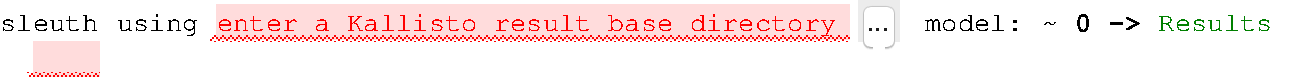
\includegraphics[width=\figWidthWide]{figures/NewSleuthStatement-1.pdf}
\caption[New Sleuth Statement.]{\textbf{New Sleuth Statement.}}
\label{fig:NewSleuthStatement}
\end{figure}

The statement has three attributes:
\paragraph{Kallisto Result Base Directory}
This is a string attribute where you can paste the path to \texttt{KALLISTO\_RESULTS}. Once pasted, if the directory contains Kallisto result sub-directories, the information is organized into a MetaR Table, that will appear in the model. An import statement is added to the analysis and the table becomes referenced by the sleuth statement. A sleuth statement bound to a table is shown in Figure~\ref{fig:KallistoBoundToTable}. At this point, you can annotate the table as you would for a Limma voom or EdgeR analysis: add column groups to columns corresponding to samples and annotate the groups with usages to define factors that you would like to include the analysis (see Chapter~\ref{chap:Tables} to learn how to do this).
For instance, using the Kallisto results from the Sleuth tutorial, the ColumnGroupContainer and Table would look as shown on Figure~\ref{fig:AnnotatedTable}.



\begin{figure}[h!tbp]
\centering
  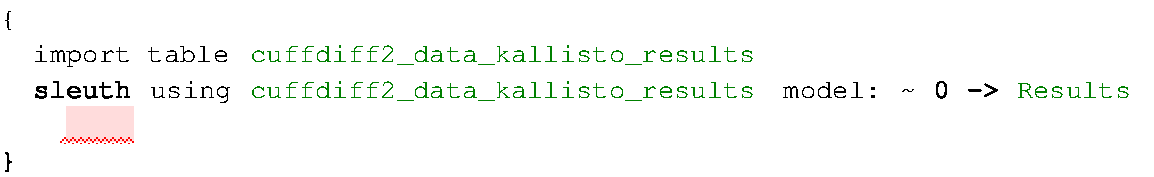
\includegraphics[width=\figWidthWide]{figures/SleuthBoundToTable-1.pdf}
\caption[Sleuth Statement Bound to a Table.]{\textbf{Sleuth Statement Bound to a Table.} The statement shown has been bound to a table by entering a valid Kallisto results directory.}
\label{fig:KallistoBoundToTable}
\end{figure}

\begin{figure}[h!tbp]
  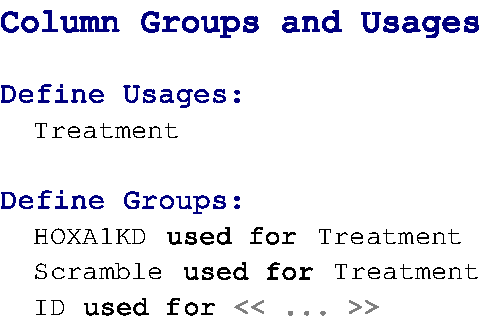
\includegraphics[width=\figWidthTiny]{figures/AnnotatedColumnGroupSleuth-1.pdf}
    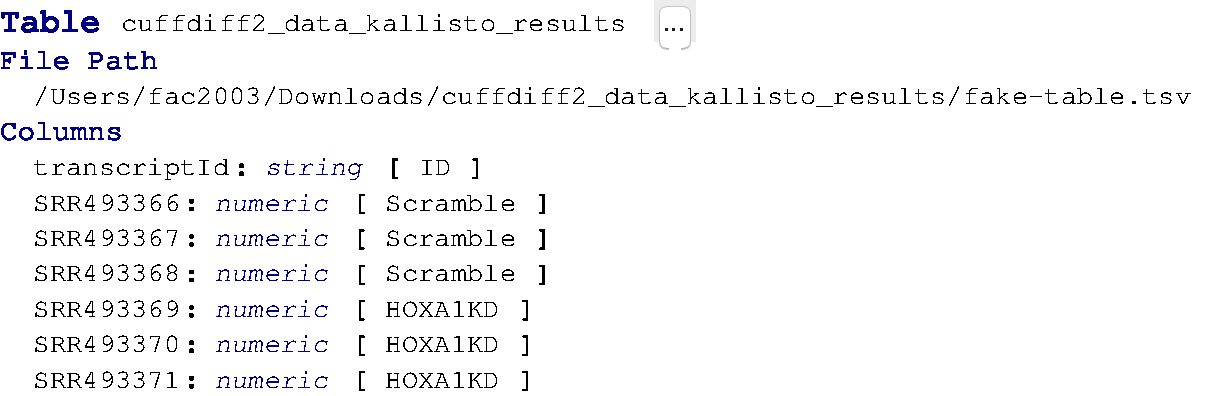
\includegraphics[width=\figWidthWide]{figures/AnnotatedTableSleuth-1.pdf}
\caption[ColumnGroup and Table for Sleuth Tutorial]{\textbf{ColumnGroup and Table for Sleuth Tutorial} Left: ColumnGroupContainer configured for the Sleuth tutorial. Right: Table imported from Kallisto base directory, and annotated with the Scramble and HOXA1KD groups.}
\label{fig:AnnotatedTable}
\end{figure}

\paragraph{Full Model}
A model attribute can be specified after \texttt{model:}. This model should represent the full set of factor/group usages you plan to use to model expression data. You need to annotate columns of the table with groups and group usage before you can use auto-completion to define the model. 

\section{Statistical Test}
The attribute shown on the second line determines the type of statistical test to perform. Sleuth supports two options at this time:
\begin{itemize}
  \item Wald test
  \item Likelihood Ratio Test (LRT)
\end{itemize}

Place the cursor over the pink cell and use auto-completion to choose one of these options. 
\paragraph{Likelihood Ratio Test}\index{LRT}\index{Likelihood Ratio Test}
If you select the LRT, you get to enter a label and a second model. The label is a text string that helps you remember what the alternate model represents. Note that Sleuth only supports an alternate model that is fully contained in the full model. This means that you can remove covariates from the alternate model, but not add some that are not present in the full model (at this time, MetaR does not check for this condition, so watch out). 

\begin{center}

\includegraphics[width=\figWidthNarrow]{figures/SleuthLRT-1.pdf}
\end{center}


\paragraph{Wald Test}\index{Wald Test}

If you select Wald Test, you get the option of entering one group and one usage. The combination should identify a condition for which you are seeking to find differentially expressed transcripts. It is unclear what the test reports when there are several levels to a factor (i.e., a group usage associated with three or more groups).

\begin{center}

\includegraphics[width=\figWidthNarrow]{figures/SleutWaldTest-1.pdf}
\end{center}